\begin{lemma}
A function f(x) is said to be convex if following inequality is true for $\lambda \in [0,1] :$  \label{opt/2/1/a/lemma1}
\begin{align}
    \lambda f(x_1) + (1-\lambda)f(x_2) \geq f(\lambda x_1 + (1-\lambda)x_2)
\end{align}
\end{lemma}

Given :
\begin{align}
    f(x) &= 4x-\frac{1}{2}x^2 , x \in \sbrak{-2,\frac{9}{2}}
\end{align}

Checking convexity of $f(x)$ :
\begin{equation}
\begin{aligned}
    &\lambda\brak{4x_1-\frac{1}{2}x_1^2} + (1-\lambda)\brak{4x_2-\frac{1}{2}x_2^2} \geq \\
    &4\brak{\lambda x_1 + (1-\lambda)x_2} - \frac{1}{2}\brak{\lambda x_1 + (1-\lambda)x_2}^2
\end{aligned}
\end{equation}

resulting in
\begin{align}
    x_1^2\brak{\frac{\lambda^2-\lambda}{2}}+x_2^2\brak{\frac{\lambda^2-\lambda}{2}}+ 2x_1x_2\brak{\frac{\lambda-\lambda^2}{2}} &\geq 0 \\
    \implies \brak{\frac{\lambda^2-\lambda}{2}}\brak{x_1^2+x_2^2-2x_1x_2} &\geq 0 \\
    \implies -\frac{1}{2}\lambda\brak{1-\lambda}\brak{x_1-x_2}^2 &\geq 0 \\
    \implies \frac{1}{2}\lambda\brak{1-\lambda}\brak{x_1-x_2}^2 &\leq 0
\end{align}

Hence,using lemma \ref{opt/2/1/a/lemma1}, given $f(x)$ is a concave function .

\begin{enumerate}
    \item For Maxima : \\
    Using gradient ascent method,
    \begin{align}
        x_{n+1} &= x_n + \alpha \nabla f(x_n) \\
        \implies x_{n+1} &= x_n + \alpha \brak{4-x_n}
    \end{align}
    
    Taking $x_0=-2,\alpha=0.001$ and precision= \\ 0.00000001,values obtained using python are:
    \begin{align}
        \boxed{\text{Maxima} = 7.999999999950196 \approx 8 }\\
        \boxed{\text{Maxima Point} = 3.9999900196756437 \approx 4}
    \end{align}
    
    
    \begin{figure}[!ht]
    \centering
    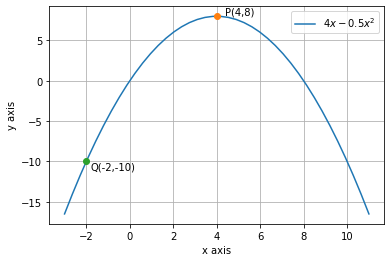
\includegraphics[width=\columnwidth]{solutions/su2021/2/1/a/Figure15.png}
    \caption{$f(x)=4x-0.5x^2$}
    \label{opt/2/1/a/f(x)}	
    \end{figure}

    \item For Minima : \\
    
    \numberwithin{table}{section}
    \begin{table}[!ht]
    \centering
    \begin{tabular}{|c|c|} 
    \hline
    $x$ & $f(x)$ \\
    \hline
    -2 & -10 \\
    \hline
    4 & 8 \\
    \hline
    4.5 & 7.875 \\
    \hline
    \end{tabular}
    \caption{Value of $f(x)$}
    \label{opt/2/1/a/tab:table1}
    \end{table}
    
    Critical point is given by
    \begin{align}
        \nabla f(x) &= 0 \\
        \implies x &= 4
    \end{align}
    
    and,end points are $x=-2$ and $x=4.5$ .
    
    Using table \ref{opt/2/1/a/tab:table1},
    \begin{align}
        \boxed{\text{Minima} = -10}\\
        \boxed{\text{Minima Point} = -2}
    \end{align}
    
\end{enumerate}



